\chapter{General Design Concepts}
\label{chapter:concepts}
%Go into detail about rules, permission, chores
In the Media-Online Management there are a few concepts that will be used through out the report. These are chore, permission and rules. The meaning of each will be explain in following sections.\fixme{Evt. refferance til intro afsnit, alt efter hvor meget det minder om hinanden. Men uanset er det godt med en opsang.}

\section{Chore}
A chore in MOM is a representation of a house chore that is to be done regularly. We have included chore into this system to encourage children to help with the house chores which gives more time for media as a reward. Therefore each chore needs a number of points which will be given when the child has done the house chore. 
An example on a house chore could be to take out the garbage, then the chore in MOM would have a name: 'take out garbage', possible a bigger description of the chore: 'remember to sort the garbage into the correct trash cans' and when the chore is done some points is given: '10'.  

One disadvantage about the chore design is that the parent needs to use the website to award the child with points for doing a chore. We would have liked to automate it further, but to limit the scope of the project this would be future work.  

\section{Permission}


%Permissions in this system is a time period in which the child user is allowed to use a specific media. Permission is included in MOM to give parents an easy way of controlling which time periods during the day the media can be used by the child. This can help the parents to get the children to bed in time since they cannot use the medias unless the parent allows it. It would especially be useful if the child has medias in his room such that the parents do not need to check whether the media is turned off or not. 

%The permission consist of:
%\begin{itemize}
	%\item a name of the permission
	%\item a representation for the time period, which would need a from time and a to time. 
	%\item a representation of days where the permission applies, which can be all days of the week or just some of them.
	%\item a representation of when it should be repeated, which can be:
		%\begin{itemize}
		%\item weekly
		%\item every second week
		%\item every third week
		%\item first in a month
		%\item last in a month
		%\end{itemize}
%\end{itemize}
%
%An example of a permission is Peter is allowed to use the TV each weekendy in the time period 17:00 to 19:00. The permission in the system would then have a time 17:00 (FromTime), a time 19:00 (ToTime), the day representation 'Saturday, Sunday', and it's repeated weekly.


\section{Rule}
\label{sec:rule}
In the system a rule can be many things the following is just a few examples of rules:

\begin{itemize}
	\item Any permissions can be written as a rule
	\item The first Monday in a month Peter's points is increased by 100
	\item Mom and Dad's profiles have unlimited time and unrestricted access to any media
\end{itemize}

The rule has been included because it gives the parents a more powerful method to control their children's use of medias. 
But there is one disadvantage with rules, it might be complicated for the user to understand how to use them. 
This means we must take care to design the concept of rules, so that it is easy to use and understand their effects.

A rule should be connected to one or more user profiles since the rules otherwise would be unnecessary. A rule consist of a name, a set of actions and  a restricted set of conditions depending on the actions. A condition is used to decide when a rule is relevant which is when all conditions fits. An action is something that can or should be done if all of the rule's conditions hold.
To see a quick overview of the different conditions and their name:

\begin{description}
	\item[Timeperiode] the action can be done in this time period. 
	\item[Timestamp] the action may only happen at a given point in time. 
	\item[Controller on] the action can be done if a specific controller is turn on. 
	\item[Controller off] the action can be done if a specific controller is turn off. 
	\item[True] The action can always be taken.
\end{description}

An overview of the actions and their name is listed below:

\begin{description}
	\item[Block user] it will block the profiles of all profiles connected to the rule.
	\item[Activate user] it will activate the profiles connected to it. 
	\item[Add points] it will add points to the profiles' points.
	\item[Delete points]  it will delete points to the profiles' points.  
	\item[Set maximum of point] it will set a maximum number of points that a profile can have. 
	\item[Unlimited time] it will give the profile unlimited time to be spend on any media. 
	\item[Access any controller] it will give the profile access to any media in the system. 
	\item[Cannot access any controller] the profile will not have access to any media. 
	\item[Access controller] it will give the profile access to a specific media. 
	\item[Cannot access controller] it will block the user from using a specific media. 
\end{description}
	
The rule's structure is presented in a grammar in listing	\ref{grammar} expressed in Extended Backus-Naur Form(EBNF) \citep{CoPL}.
In a nonterminal is en-captured in $<>$ and a terminal is just a word or en-captured in "". 
Also the grouping is used represented in $()$, the replica symbol is $*$, comments is $(**)$ and alternative is $|$. 

A rule consist of a name and one of five action and condition sets which determine which actions and conditions can be combined. A rule can have several actions and conditions but only from the same set, see line 1-7. The action set is presented from 9-23 where all has a specific name, some have a specific Controller represented as a number and some has points which is a number. The condition set likewise represented from 9-23 and the condition types are presented from 25-30. There are four types but they each have a specific name. One type has Timestamp, another a Controller, the third only the name and the last is a timeperiod. The timeperiod has with two timestamp and if it is repeatable it has a string representation of the weekdays and a representation of then it is repeatable. 

\begin{lstlisting}[label=grammar, caption=Grammar of a rule in EBNF]
<Rule>:= <name> (
	 	  (<ActionsetSet1><ConditionSet1>)*
		| (<ActionsetSet2><ConditionSet2>)*
		| (<ActionsetSet3><ConditionSet3>)*
		| (<ActionsetSet4><ConditionSet4>)*
		| (<ActionsetSet5><ConditionSet5>)*
	)

<ActionsetSet1> := "Block user" | "Activate user" 
<ConditionSet1> := <ConditionTimestamp>

<ActionsetSet2> := ("Add points" | "Delete points") <Points>
<ConditionSet2> := <ConditionTimeperiod> | <ConditionTimestamp>

<ActionsetSet3> := "Set maximum of point" <Points>
<ConditionSet3> := <ConditionTrue>

<ActionsetSet4> := "Unlimited time" | ("Access any controller" | "Cannot access any controller") <Controller>
<ConditionSet4> := <ConditionTimeperiod> | <ConditionTimestamp> 

<ActionsetSet5> := ("Access controller" | "Cannot access controller")<Controller>
<ConditionSet5> := <ConditionTimestamp> |	<ConditionTimeperiod> 
					| 	<ConditionTrue>	|	<ConditionElse>	
				
<ConditionTimestamp> :=  "Timestamp" <Timestamp>
<ConditionTimeperiod> :=  "TimePeriod" <Timestamp> <Timestamp> <Repeatable>					
<Repeatable> :=   <Weekdays> <Repeat> | Nill

<ConditionTrue> := "True" 
<ConditionElse>:= ("Device on" | "Device off") <Controller>
				
<Name> := ALPHA*  (* Upper and lowercase ASCII letters (A-Z,a-z) *)
<Controller> := DIGIT* (* Decimal digits (0-9) *)
<Points> := DIGIT*
<Timestamp> := 4*DIGIT,"-",2*DIGIT,"-",2*DIGIT, " ",2*DIGIT,":"2*DIGIT,":"2*DIGIT  (*YYYY-MM-DD HH:mm:ss*)
<Weekdays> := ("monday"| "tuesday"| "wednesday"| "thursday"| "friday"| "saturday"| "sunday")*
<Repeat> := "weekly" | "biweekly" | "triweekly" | "first in month" | "last in month"
\end{lstlisting}
		

\subsection{Permission and Rules Precedence}
It should be possible to override permissions and rules with another rule, but then some priority rules  need to be established. 
For the overriding of the two to be relevant they need to overlap in time which mean that the condition should use Timeperiod or True. Also if it is a rule then it should have an action with the name 'Cannot access controller', 'Access controller', 'Cannot access any controller' or 'Access any controller' to be relevant. So from the grammar \ref{grammar} it is the rule sets $<name> <ActionsetSet4><ConditionSet4>$  and $<name> <ActionsetSet5><ConditionSet5>$ that need the priority.

We came to the conclusion that rules always have precedence over permissions. But if the conflict is among two rules it is a more complex set of precedence rules. First to determine the precedence we look at the action's name. See figure \ref{fig:precendence} where the precedence graph is shown. Notice that the precedence for 'Cannot access controller' and 'Access controller' can be either way depending on the condition. Otherwise both of them has priority over 'Access any controller' which also has priority over 'Cannot access any controller'. 
  
\begin{figure}
	\centering
		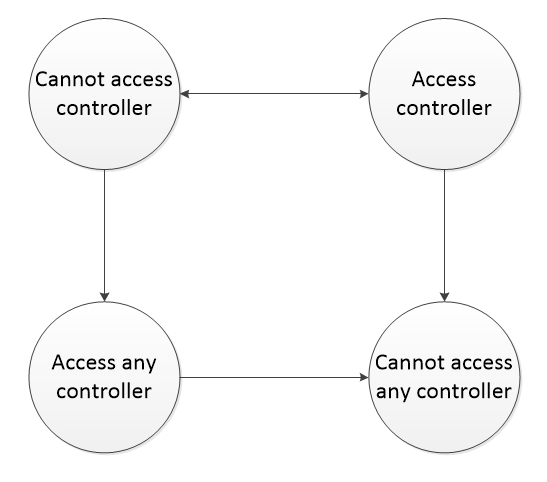
\includegraphics[width=0.75\textwidth]{images/precendence.jpg}
	\caption{Precedence of rules}
	\label{fig:precendence}
\end{figure}

When the condition determines the precedence we have different combinations:

\begin{itemize}
	\item If one is True and the other is Timeperiod then the rule with the Timeperiod has the higher precedence
	\item If both is True then Access controller has the precedence.
	\item If both is Timeperiod:
		\begin{itemize}
			\item If both is repeatable or non-repeatable then Access controller has the precedence
			\item If one is repeatable and the other is nonrepeatable then the rule with the nonrepeatable Timeperiod has the higher precedence.
		\end{itemize}
\end{itemize}

These precedence rules do not avoid all possible conflict but it limits them.  
	
\subsubsection{Examples of Rules}
In this section some examples of rules for a profile will be given.

The first example could be that the profile Peter gets point for each football training and the football training is Monday and Thursday from 18:00 to 19:30 each week. Then the action could be add 25 points to Peter when condition holds. The condition is from 19:30 to 19:30 where the day is 'Monday, Thursday' and it is repeated weekly. \\

The second example could be that Susan is grounded from the 2nd December. In the system there will be a condition with Timestamp which is 2nd December 2013 18:00
and an action that is 'Block user' such that she cannot use any media or gain points in this period. \\

If the parents should make a rule which give themselves unlimited time and access to any media. The condition would be True and the actions would be 'Unlimited time' and 'Access any controller'.\\\\

This conclude the general concepts that will be used through out the remainder of the report. Next further details about the requirements of MOM is described.  

%
%\section{General Design Concepts}
%%Go into detail about rules, permission, chores
%In the Media-Online Management there are a few concepts that will be used through out the report. These are chore, permission and rules. The meaning of each will be explain in following sections.\fixme{Evt. refferance til intro afsnit, alt efter hvor meget det minder om hinanden. Men uanset er det godt med en opsang.}
%
%\subsection{Chore}
%A chore in MOM is a representation of a house chore that is to be done regularly. We have included chore into this system to encourage children to help with the house chores which gives more time for media as a reward. Therefore each chore needs a number of points which will be given when the child has done the house chore. 
%An example on a house chore could be to take out the garbage, then the chore in MOM would have a name: 'take out garbage', possible a bigger description of the chore: 'remember to sort the garbage into the correct trash cans' and when the chore is done some points is given: '10'.  
%
%One disadvantage about the chore design is that the parent needs to use the website to award the child with points for doing a chore. We would have liked to automate it further, but to limit the scope of the project this would be future work.  
%
%\subsection{Permission}
%Permissions in this system is a time period in which the child user is allowed to use a specific media. Permission is included in MOM to give parents an easy way of controlling which time periods during the day the media can be used by the child. This can help the parents to get the children to bed in time since they cannot use the medias unless the parent allows it. It would especially be useful if the child has medias in his room such that the parents do not need to check whether the media is turned off or not. 
%
%The permission consist of:
%\begin{itemize}
	%\item a name of the permission
	%\item a representation for the time period, which would need a from time and a to time. 
	%\item a representation of days where the permission applies, which can be all days of the week or just some of them.
	%\item a representation of when it should be repeated, which can be:
		%\begin{itemize}
		%\item weekly
		%\item every second week
		%\item every third week
		%\item first in a month
		%\item last in a month
		%\end{itemize}
%\end{itemize}
%
%An example of a permission is Peter is allowed to use the TV each weekday in the time period 17:00 to 19:00. The permission in the system would then have a time 17:00 (FromTime), a time 19:00 (ToTime), the day representation 'Monday, Tuesday, Wednesday, Thursday, Friday', and it's repeated weekly.\fixme{M�ske lidt for meget Database representation med Monday, Tuesdag...}
%
%
%\subsection{Rule}
%In the system a rule can be many things the following is just a few examples of rules:
%
%\begin{itemize}
	%\item any permission can also be written as a rule
	%\item The first Monday in a month increase Peter's points by 100
	%\item Mom and Dad's profiles have unlimited time and unrestricted access to any media
%\end{itemize}
%
%The rule has been included because it gives the parent users more powerful methods to control the use of medias in MOM. %and to control the profiles in the 
%But there is one disadvantage with rules, it might be complicated for the user to understand how to use them. 
%This means we must take care to design the concept of rules, so that it is easy to use and understand their effects.
%%and how to construct a rule so the design of how the user can make a rule need to be though through carefully.
%
%A rule should be connected to one or more user profiles since the rules otherwise would be unnecessary if no one should follow them. A rule consist of a name, a set of conditions and a set of actions. The conditions and actions will be explained further in the following sections.
	%
%\subsubsection{Condition}
%A condition is used to decide when a rule is relevant which is when all conditions fits. A condition has a predefine name and when the user make a condition he will choose it from a list. The names is listed below together with the additional information that is required. 
%
%\begin{description}
	%\item[Timeperiode] when this is chosen the user can define a time period. It needs the same information as a permission, a from time, a to time, representation of days where the rule applies, and a representation of when it should be repeated. The time period can be either repeatable or nonrepeatable where the from time and to time is the only data required.
	%\item[Timestamp] the condition has a timestamp as an additional information and an action should happen immediately after this timestamp have been reached. 
	%\item[Controller on] this should check whether a given controller for a media is active. This needs to be connected to a controller.
	%\item[Controller off] this should check whether a given controller for a media is not active. This needs to be connected to a controller.
	%\item[True] This is always true.
%\end{description}
%
%Later in this chapter there will be some examples of rules which uses conditions.
%
%\subsubsection{Action}
%\label{subsubsection:action}
%An action is something that can or should be done if all of the rule's conditions hold. An action always has a name, but as with the condition this name is not user defined. The user have a choice from a list which can be found in the description below with an explanation of what it does and what other information is needed for the action and which conditions it can be combined with.   
%
%\begin{description}
	%\item[Block user] it will block the profiles of all profiles connected to the rule. This action can be combined with Timestamp.
	%\item[Activate user] it will activate or re-activate the profiles of all profiles connected to the rule. This action can be combined with Timestamp.
	%\item[Add points] it will add points to all profiles connected to the rule. Here the number of points is needed. This action can be combined with Timestamp, Timeperiod(Repeateble).
	%\item[Remove points]    This action can be combined with Timestamp, Timeperiod(Repeateble).
	%\item[Set maximum of point] it will set a maximum for the number of points that a profile can have. Here a number representing the maximum points is also needed. This action can be combined with True.
	%\item[Unlimited time] it will give the profile unlimited time to be spend on any media. This action can be combined with True and Timeperiod both repeatable and nonrepeatable.
	%\item[Access any controller] it will give the profile access to any media in the system. This action can be combined with True and Timeperiod both repeatable and nonrepeatable.
	%\item[Cannot access any controller] it will not give the profile access to any media. This action can be combined with True and Timeperiod both repeatable and nonrepeatable.
	%\item[Access controller] it will give the profile access to a specific media. Here a controller need to be connected to the action. This action can be combined with any of the condition names.
	%\item[Cannot access controller] it will block the user from using a specific media. Here a controller need to be connected to the action. This action can be combined with any of the condition names.
%\end{description}
		%
%Since some of the action like 'Add points' should be done automatically without further contact with the user. A background process typically called daemon, is also needed in MOM but this will be explained further in section \ref{subsec:daemon}. 
%
%
